%%%%%%%%%%%%%%%%%%%%%%%%%%%%%%%%%%%%%%%%%%%%%%%%%%%%%%%%%%%%%%%%%%%%%%%%%%%%%%%
%                       CARGA DE LA CLASE DE DOCUMENTO                        %
%%%%%%%%%%%%%%%%%%%%%%%%%%%%%%%%%%%%%%%%%%%%%%%%%%%%%%%%%%%%%%%%%%%%%%%%%%%%%%%

\documentclass[11pt,spanish,listoffigures,listoftables]{tfgetsinf}

%%%%%%%%%%%%%%%%%%%%%%%%%%%%%%%%%%%%%%%%%%%%%%%%%%%%%%%%%%%%%%%%%%%%%%%%%%%%%%%
%                          CODIFICACIÓN DEL FICHERO                           %
%%%%%%%%%%%%%%%%%%%%%%%%%%%%%%%%%%%%%%%%%%%%%%%%%%%%%%%%%%%%%%%%%%%%%%%%%%%%%%%

\usepackage[utf8]{inputenc} 
\usepackage{babel}
\usepackage{hyperref}
\usepackage{biblatex}
\usepackage{amsmath, amssymb}
\usepackage{graphicx}
\usepackage{booktabs}
\usepackage{listings}
\usepackage{xcolor}
\usepackage{multirow}
\usepackage{subcaption}

 

\addbibresource{bib.bib}  % Enlazar el archivo .bib
\addglobalbib{bib.bib}
\hypersetup{ colorlinks=true, linkcolor=black, urlcolor=cyan }

%%%%%%%%%%%%%%%%%%%%%%%%%%%%%%%%%%%%%%%%%%%%%%%%%%%%%%%%%%%%%%%%%%%%%%%%%%%%%%%
%                             OTROS PAQUETES                                  %
%%%%%%%%%%%%%%%%%%%%%%%%%%%%%%%%%%%%%%%%%%%%%%%%%%%%%%%%%%%%%%%%%%%%%%%%%%%%%%%
% (Aquí puedes añadir los paquetes que necesites)

%%%%%%%%%%%%%%%%%%%%%%%%%%%%%%%%%%%%%%%%%%%%%%%%%%%%%%%%%%%%%%%%%%%%%%%%%%%%%%%
%                         DATOS DEL TRABAJO                                   %
%%%%%%%%%%%%%%%%%%%%%%%%%%%%%%%%%%%%%%%%%%%%%%%%%%%%%%%%%%%%%%%%%%%%%%%%%%%%%%%

\title{Clasificación automática de artrosis en rodillas mediante redes neuronales convolucionales}
\author{Hernández Martínez, Carlos}
\tutor{Juan Ciscar, Alfonso}
\curs{2024-2025}

%%%%%%%%%%%%%%%%%%%%%%%%%%%%%%%%%%%%%%%%%%%%%%%%%%%%%%%%%%%%%%%%%%%%%%%%%%%%%%%
%            PALABRAS CLAVE Y RESÚMENES (en tres idiomas)                     %
%%%%%%%%%%%%%%%%%%%%%%%%%%%%%%%%%%%%%%%%%%%%%%%%%%%%%%%%%%%%%%%%%%%%%%%%%%%%%%%

\keywords{Palabras clave en catalán} % catalán
         {Palabras clave en español} % español
         {Keywords in English}       % inglés

% Añade esto en el preámbulo (antes de \begin{document})
\setcounter{tocdepth}{1} % Muestra solo capítulos y secciones en el índice
\begin{document}

%%%%%%%%%%%%%%%%%%%%%%%%%%%%%%%%%%%%%%%%%%%%%%%%%%%%%%%%%%%%%%%%%%%%%%%%%%%%%%%
%                             RESÚMENES                                       %
%%%%%%%%%%%%%%%%%%%%%%%%%%%%%%%%%%%%%%%%%%%%%%%%%%%%%%%%%%%%%%%%%%%%%%%%%%%%%%%

\begin{abstract}
Aquí citamos a un datajkjkset \cite{gornale2020digital}.
Citación paper IEE \cite{10863523}, Dataset \cite{chen2018knee}
aqui citamos un paper \cite{VAATTOVAARA2025100580}
otra cita \cite{comprehensive_review}

Quitar imagenes brillantes -> \cite{efficientnet_paper}
\end{abstract}

\begin{abstract}[spanish]
(Resumen en castellano)
\end{abstract}

\begin{abstract}[english]
(Resumen en inglés)
\end{abstract}

\mainmatter

%%%%%%%%%%%%%%%%%%%%%%%%%%%%%%%%%%%%%%%%%%%%%%%%%%%%%%%%%%%%%%%%%%%%%%%%%%%%%%%
%                              CAPÍTULO 1                                     %
%                                    INTRO                                     %
%%%%%%%%%%%%%%%%%%%%%%%%%%%%%%%%%%%%%%%%%%%%%%%%%%%%%%%%%%%%%%%%%%%%%%%%%%%%%%%

\chapter{Introducción}  % ~5 páginas

\section{Motivación}     % 1.1
La artritis es una de las enfermedades musculoesqueléticas más prevalentes a nivel mundial y una de las principales causas de discapacidad en adultos mayores. Su diagnóstico y seguimiento se basa tradicionalmente en la evaluación clínica y en la interpretación de imágenes médicas, como radiografías, resonancias magnéticas y tomografías computarizadas. Sin embargo, este proceso suele depender en gran medida de la experiencia del profesional médico, lo que puede generar variabilidad en los diagnósticos y retrasos en la detección temprana de la enfermedad.

En los últimos años, los avances en inteligencia artificial, y en particular en el aprendizaje profundo, han demostrado un gran potencial para mejorar la precisión y la eficiencia en el análisis de imágenes médicas. Las redes neuronales convolucionales (CNN) han sido ampliamente utilizadas en el campo de la visión por computadora para tareas como la detección de patologías en radiografías, la segmentación de tejidos en resonancias magnéticas y la clasificación de niveles de severidad en enfermedades degenerativas.

Este Trabajo de Fin de Grado (TFG) se motiva por la necesidad de desarrollar métodos automáticos y robustos para el análisis de la artritis mediante el uso de técnicas de aprendizaje profundo. En particular, se busca explorar el uso de redes neuronales para la clasificación de imágenes médicas, utilizando bases de datos estandarizadas como \textit{Mendeley dataset} \cite{chen2018knee}. La aplicación de estos modelos podría no solo optimizar el proceso de diagnóstico, sino también contribuir al desarrollo de herramientas de soporte a la decisión clínica, facilitando una intervención más temprana y personalizada para los pacientes.

La relevancia de este estudio radica en su potencial impacto en la práctica clínica. Un sistema basado en inteligencia artificial podría reducir la carga de trabajo de los especialistas, mejorar la objetividad del diagnóstico y ofrecer segundas opiniones automáticas que complementen la evaluación médica tradicional. Además, el desarrollo de estas tecnologías en el ámbito de la artritis podría sentar un precedente para su aplicación en otras enfermedades musculoesqueléticas, ampliando el alcance del aprendizaje profundo en el campo de la salud.

Además, se plantea la posibilidad de realizar \textit{transfer learning} utilizando modelos preentrenados en artritis humana para aplicarlos en el diagnóstico de artritis en gatos. Esta adaptación podría beneficiar la práctica veterinaria, proporcionando herramientas automatizadas para la evaluación de la enfermedad en animales y mejorando la precisión en su diagnóstico.

En este contexto, el presente trabajo busca contribuir al avance del uso de inteligencia artificial en la detección y análisis de la artritis, evaluando diferentes enfoques de redes neuronales y analizando su rendimiento en la clasificación de imágenes médicas. La motivación principal es demostrar la viabilidad y efectividad de estos modelos en un problema biomédico concreto, promoviendo la integración de tecnologías emergentes en el ámbito de la salud.


\section{Objetivos}      % 1.2
% Presenta aquí los 3 objetivos principales
% p.e. Objetivo 1, Objetivo 2, Objetivo 3

\section{Estructura del documento}  % 1.3
% Describe la organización de los capítulos y secciones

%%%%%%%%%%%%%%%%%%%%%%%%%%%%%%%%%%%%%%%%%%%%%%%%%%%%%%%%%%%%%%%%%%%%%%%%%%%%%%%
%                              CAPÍTULO 2                                     %
%                                PRELIMINARES (STANDBY)                       %
%%%%%%%%%%%%%%%%%%%%%%%%%%%%%%%%%%%%%%%%%%%%%%%%%%%%%%%%%%%%%%%%%%%%%%%%%%%%%%%

\chapter{Preliminares}  % ~15 páginas
\section{Aprendizaje automático}
El \textbf{aprendizaje automático} es una rama de la inteligencia artificial que se enfoca en que las máquinas mejoren 
su desempeño en una tarea determinada a partir de la experiencia. Un sistema \textit{“aprende”} cuando su desempeño en una tarea, 
medido por una métrica, mejora con la experiencia adquirida. En términos prácticos, esto implica diseñar algoritmos capaces de 
\textit{generalizar} patrones a partir de datos, de forma que puedan hacer predicciones o tomar decisiones sobre datos no vistos 
previamente. En aprendizaje automático se suelen representar los datos con un conjunto de \textit{características} (features) relevantes, y el algoritmo 
construye un modelo matemático que relaciona estas características con las salidas esperadas. Un objetivo central es lograr un buen 
equilibrio entre \textit{ajuste} a los datos de entrenamiento y \textit{capacidad de generalización} a nuevos datos, evitando problemas 
como el \textit{sobreajuste} (overfitting).

Existen varias categorías principales de aprendizaje automático, diferenciadas por la forma en que el algoritmo recibe la información 
y el tipo de tarea a resolver:

\begin{itemize}
    \item \textbf{Aprendizaje supervisado}: El algoritmo recibe ejemplos de entrada y su correspondiente salida deseada (etiquetas). 
    El objetivo es aprender una función que mapee las entradas a las salidas correctas. Son tareas típicas la \textit{clasificación} 
    (p. ej., dado un conjunto de características de un paciente, predecir si tiene una enfermedad: salida categórica) y la 
    \textit{regresión} (p. ej., predecir un valor numérico como el precio de una casa). El rendimiento se evalúa comúnmente con métricas
    como la exactitud en clasificación o el error cuadrático medio en regresión.

    \item \textbf{Aprendizaje no supervisado}: El algoritmo recibe datos de entrada sin etiquetas, y debe descubrir estructura oculta en 
    ellos. Incluye tareas como la \textit{clustering} (agrupamiento de datos por similitud) o la \textit{reducción de dimensionalidad} 
    (encontrar representaciones más compactas de los datos). Por ejemplo, un algoritmo no supervisado podría agrupar automáticamente 
    imágenes médicas en tipos similares sin conocer de antemano las patologías presentes.
    
    \item \textbf{Aprendizaje por refuerzo}: El algoritmo (un \textit{agente}) aprende a través de la interacción con un entorno, 
    recibiendo recompensas o penalizaciones según sus acciones. El agente debe descubrir una política de acciones que maximice la 
    recompensa acumulada. Este paradigma es común en robótica y juegos, donde no se proporcionan ejemplos de solución directa sino una 
    señal de calidad de cada acción.
    
\end{itemize}

El proceso típico de aprendizaje supervisado consiste en entrenar un modelo ajustando sus parámetros para minimizar un 
\textit{funcional de coste} (que mide el error de las predicciones del modelo sobre los datos de entrenamiento). El procedimiento de 
optimización más difundido es el \textit{descenso de gradiente} y sus variantes (p. ej., descenso de gradiente estocástico para procesar 
por lotes de ejemplos). En cada iteración, se calcula la gradiente del error respecto a los parámetros del modelo, y se ajustan los 
parámetros en la dirección opuesta a dicha gradiente para reducir el error. Este ciclo se repite múltiples veces (\textit{épocas}) 
hasta converger a un mínimo (generalmente un mínimo local del error). El pseudocódigo en el Algoritmo \ref{alg:gd-train} ilustra este 
proceso de manera simplificada para un modelo supervisado entrenado mediante descenso de gradiente.

\begin{algorithmic}
    \label{alg:gd-train}
    \REQUIRE Conjunto de entrenamiento ${(x_i, y_i)}_{i=1}^N$, tasa de aprendizaje $\eta$ función de error $\mathcal{L}$
    \STATE Inicializar parámetros del modelo $\theta$ (p. ej. aleatoriamente)
    \FOR{numero de épocas}
        \FOR{cada $(x_i, y_i)$ en ${(x_i, y_i)}_{i=1}^N$}
            \STATE calcular predicción $\hat{y}_i = f_\theta(x_i)$
            \STATE calcular pérdida $L = \mathcal{L}(\hat{y}_i, y_i)$ \COMMENT{ej.: error cuadrático, entropía cruzada, etc.}
            \STATE calcular gradiente $g = \nabla_{\theta} L$
            \STATE actualizar parámetros: $\theta := \theta - \eta \cdot g$
        \ENDFOR
    \ENDFOR
\end{algorithmic}

\section{Apr}

El aprendizaje automático (\textit{Machine Learning, ML}) es una rama de la inteligencia artificial que se centra en el 
desarrollo de algoritmos y modelos capaces de aprender a partir de datos. Esta tecnología ha transformado múltiples 
disciplinas al permitir que los sistemas mejoren su desempeño en tareas específicas mediante la experiencia, sin requerir 
una programación explícita para cada situación. Desde sus orígenes en técnicas estadísticas básicas hasta los modernos 
enfoques de aprendizaje profundo, ML ha evolucionado significativamente, impulsado por el incremento en la disponibilidad 
de datos y el avance en capacidad computacional. 

\begin{figure}[htbp]
    \centering
    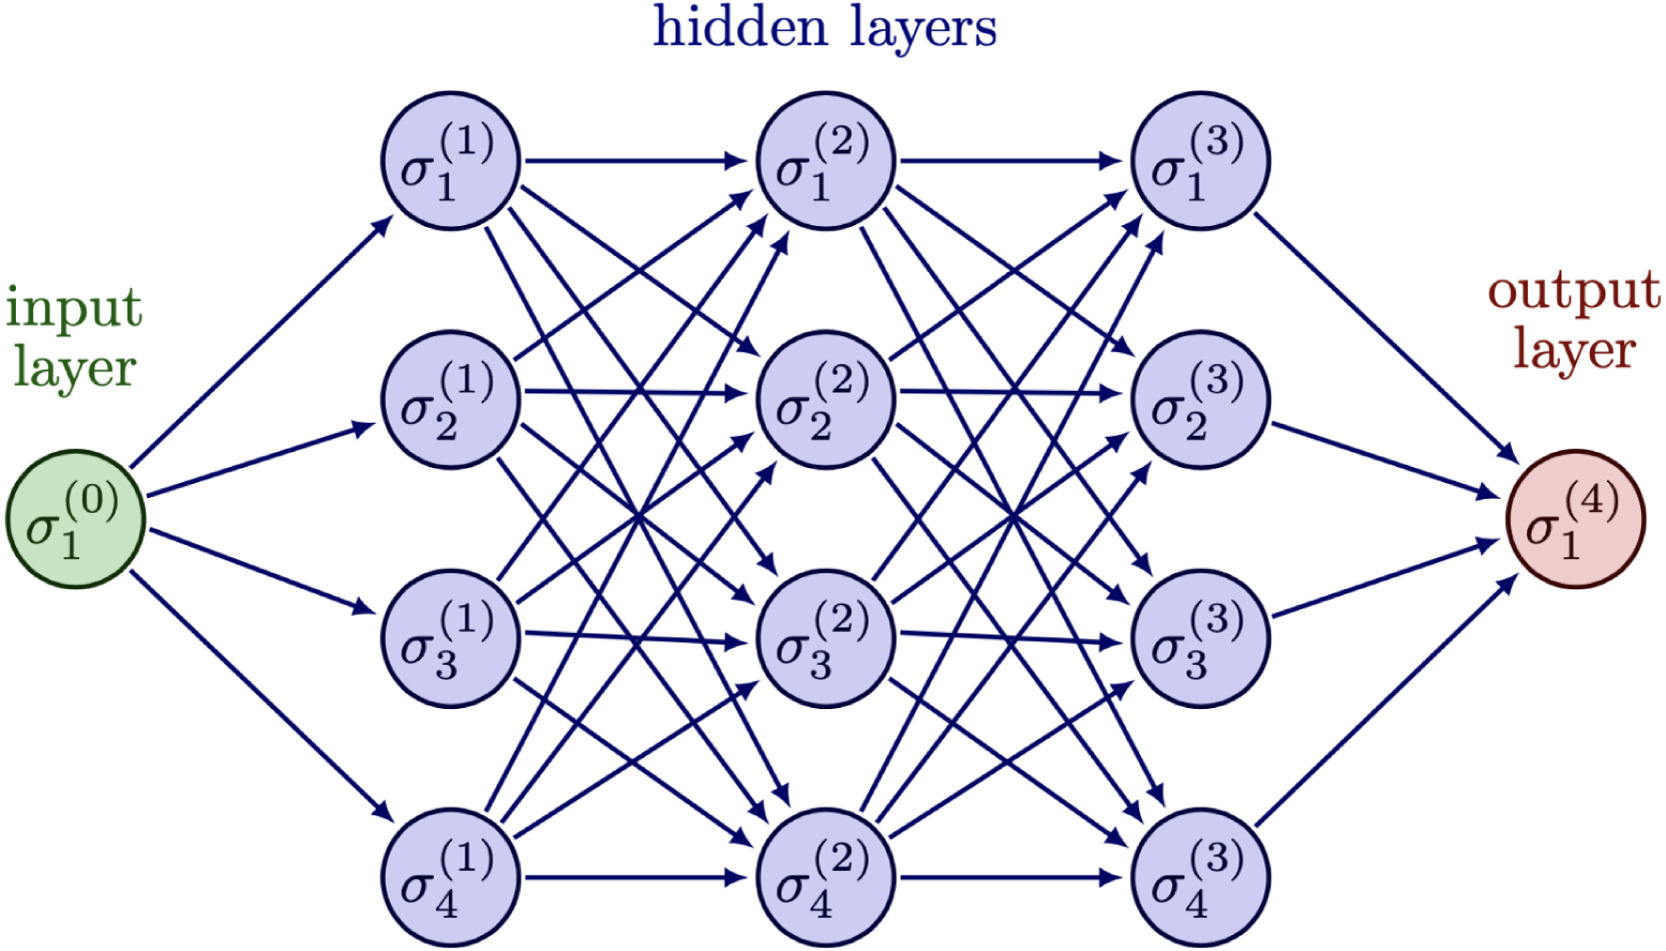
\includegraphics[width=0.7\textwidth]{neural_network.jpg}
    \caption{Ejemplo de una red neuronal profunda \cite{neural_network}}
    \label{fig:mi_imagen}
  \end{figure}
\subsection{Categorías de Aprendizaje Automático}

El aprendizaje automático se puede clasificar en tres paradigmas fundamentales:

\begin{itemize}
    \item \textbf{Aprendizaje supervisado}: Este enfoque utiliza conjuntos de datos etiquetados para entrenar modelos que aprendan a mapear entradas a salidas correctas. Algoritmos comunes en este paradigma incluyen la regresión lineal, las máquinas de soporte vectorial (SVM) y las redes neuronales profundas. 
    % //IMAGEN: Diagrama de flujo del proceso de aprendizaje supervisado.
    
    \item \textbf{Aprendizaje no supervisado}: En este caso, los datos no cuentan con etiquetas, y el objetivo es descubrir estructuras subyacentes o patrones en el conjunto de datos. Se emplean técnicas como el clustering, el análisis de componentes principales (PCA) y modelos generativos.
    % //IMAGEN: Ejemplo visual de un algoritmo de clustering aplicado a datos.
    
    \item \textbf{Aprendizaje por refuerzo}: Aquí, un agente interactúa con su entorno, tomando decisiones basadas en un sistema de recompensas y penalizaciones. A través de la retroalimentación, el agente aprende a optimizar su comportamiento para maximizar la función de recompensa.
    % //IMAGEN: Esquema que muestra el ciclo de interacción en el aprendizaje por refuerzo.
\end{itemize}

\subsection{Procesamiento de Datos en Aprendizaje Automático}

La calidad de los datos de entrada es determinante para el rendimiento y la capacidad de generalización de un modelo de ML. Por ello, el procesamiento de datos abarca varias fases esenciales:

\begin{itemize}
    \item \textbf{Preprocesamiento}: Consiste en la limpieza, normalización y transformación de los datos para eliminar ruidos y gestionar valores faltantes. En el caso de imágenes médicas, este proceso puede incluir la corrección de artefactos, la estandarización de intensidades y la segmentación preliminar de regiones de interés.
    % //IMAGEN: Diagrama que ilustra el flujo de preprocesamiento en imágenes médicas.
    
    \item \textbf{División del conjunto de datos}: Se segmenta la información en subconjuntos de entrenamiento, validación y prueba. Esta división es crucial para ajustar los hiperparámetros del modelo, prevenir el sobreajuste y evaluar de forma objetiva el desempeño final.
    % //IMAGEN: Representación gráfica de la partición de datos en entrenamiento, validación y test.
    
    \item \textbf{Extracción y selección de características}: En algunos casos, es necesario identificar y extraer características relevantes que potencien la capacidad del modelo para detectar patrones significativos, especialmente en dominios de alta dimensionalidad.
\end{itemize}

\subsection{Métricas de Evaluación}

La evaluación del rendimiento de los modelos de aprendizaje automático se realiza mediante diversas métricas, que varían según la naturaleza del problema:

\begin{itemize}
    \item \textbf{Para clasificación}: Se utilizan métricas como la precisión (\textit{accuracy}), la precisión (precision), la sensibilidad (recall) y el F1-score. La curva ROC y el área bajo la curva (AUC-ROC) también son fundamentales para evaluar la capacidad del modelo para distinguir entre clases.
    % //IMAGEN: Ejemplo gráfico de una curva ROC con el cálculo del AUC.
    
    \item \textbf{Para regresión}: Se emplean métricas como el error cuadrático medio (MSE) y el error absoluto medio (MAE), que cuantifican la diferencia entre las predicciones y los valores reales.
\end{itemize}

\subsection{Aplicaciones del Aprendizaje Automático en Imágenes Médicas}

La integración de ML en el análisis de imágenes médicas ha permitido avances significativos en el campo del diagnóstico y la intervención clínica. Entre las aplicaciones más relevantes se encuentran:

\begin{itemize}
    \item \textbf{Detección de enfermedades}: Modelos supervisados permiten identificar anomalías en diversos tipos de imágenes médicas, facilitando diagnósticos tempranos y precisos.
    % //IMAGEN: Ejemplo de radiografía con áreas destacadas que indican anomalías.
    
    \item \textbf{Segmentación de tejidos y órganos}: Las redes neuronales, especialmente las CNN, posibilitan la delimitación precisa de regiones de interés, lo cual es esencial para planificar tratamientos y procedimientos quirúrgicos.
    % //IMAGEN: Imagen segmentada de una resonancia magnética mostrando la delimitación de órganos.
    
    \item \textbf{Clasificación de tumores}: Los modelos de aprendizaje profundo pueden diferenciar entre tumores benignos y malignos, proporcionando una segunda opinión automatizada que complementa la evaluación clínica.
\end{itemize}

\subsection{Ventajas, Desafíos y Perspectivas Futuras}

El aprendizaje automático ofrece múltiples ventajas en el ámbito médico, aunque también presenta desafíos que requieren atención:

\begin{itemize}
    \item \textbf{Ventajas}:
    \begin{itemize}
        \item Automatización del análisis de grandes volúmenes de datos.
        \item Capacidad para detectar patrones complejos y no lineales.
        \item Reducción de la variabilidad interobservador en el diagnóstico.
    \end{itemize}
    % //IMAGEN: Tabla comparativa de las ventajas del aprendizaje automático en imágenes médicas.
    
    \item \textbf{Desafíos}:
    \begin{itemize}
        \item La necesidad de contar con grandes volúmenes de datos etiquetados.
        \item Riesgo de sobreajuste y la necesidad de aplicar técnicas de regularización.
        \item Problemas de interpretabilidad, lo que puede dificultar la adopción en entornos clínicos.
    \end{itemize}
    % //IMAGEN: Diagrama que ilustra los desafíos del sobreajuste y la interpretabilidad en ML.
    
    \item \textbf{Perspectivas Futuras}:
    La investigación en ML continúa avanzando hacia modelos más robustos y explicables. El desarrollo de técnicas de transferencia de aprendizaje, la integración de algoritmos híbridos y el fomento de la interpretabilidad serán clave para una mayor adopción en el ámbito médico, permitiendo sistemas de apoyo al diagnóstico cada vez más precisos y confiables.
    % //IMAGEN: Esquema que presenta las tendencias futuras en el desarrollo de ML para aplicaciones médicas.
\end{itemize}

En resumen, el aprendizaje automático representa una herramienta poderosa que, a través de su continua evolución, promete revolucionar el análisis de imágenes médicas. Su capacidad para automatizar y mejorar procesos diagnósticos no solo optimiza la eficiencia clínica, sino que también abre la puerta a un futuro en el que la inteligencia artificial se integre de manera efectiva en la toma de decisiones médicas.


\section{Redes neuronales}
Las redes neuronales son modelos computacionales inspirados en el funcionamiento del cerebro humano, diseñados para reconocer patrones y aprender representaciones a partir de datos. Su capacidad para aproximar funciones complejas las ha convertido en una herramienta fundamental en el ámbito del aprendizaje profundo y el análisis de imágenes médicas.

\subsection{Estructura y Funcionamiento}
Una red neuronal se compone de varias capas de neuronas artificiales:
\begin{itemize}
    \item \textbf{Capa de entrada:} Recibe los datos iniciales y los distribuye a las neuronas de las capas siguientes.
    \item \textbf{Capas ocultas:} Una o varias capas intermedias que transforman las entradas mediante combinaciones lineales y funciones de activación no lineales, permitiendo la extracción de características relevantes.
    \item \textbf{Capa de salida:} Genera la respuesta final del modelo, que puede corresponder a una clasificación, una regresión u otra tarea específica.
\end{itemize}
Cada neurona realiza una suma ponderada de sus entradas, seguida de la aplicación de una función de activación (por ejemplo, sigmoide, ReLU o tanh), lo que introduce la no linealidad necesaria para modelar relaciones complejas.

\subsection{Proceso de Aprendizaje y Optimización}
El aprendizaje en redes neuronales se basa en la minimización de una función de coste, que cuantifica la diferencia entre las predicciones del modelo y los valores reales. Este proceso se lleva a cabo mediante:
\begin{itemize}
    \item \textbf{Backproping:} Algoritmo que permite calcular el gradiente del error con respecto a cada peso en la red, facilitando su ajuste.
    \item \textbf{Descenso de gradiente:} Método de optimización utilizado para actualizar los pesos de forma iterativa y reducir la función de coste.
\end{itemize}
El éxito del aprendizaje depende, en gran medida, de la elección de la función de activación, la arquitectura de la red y los hiperparámetros del algoritmo de optimización.

\subsection{Principales Arquitecturas de Redes Neuronales}
Existen diversas configuraciones de redes neuronales, cada una adaptada a distintos tipos de problemas:
\begin{itemize}
    \item \textbf{Redes Feedforward:} La información fluye en una única dirección desde la entrada hasta la salida, siendo las más simples en estructura.
    \item \textbf{Redes Convolucionales (CNN):} Especializadas en el procesamiento de datos con estructura de grilla, como imágenes. Su uso es fundamental en tareas de visión por computadora, donde permiten extraer características espaciales relevantes.
    \item \textbf{Redes Recurrentes (RNN):} Diseñadas para trabajar con datos secuenciales, en las que la información de estados anteriores influye en las predicciones actuales.
\end{itemize}

\subsection{Aplicaciones en Imágenes Médicas}
En el análisis de imágenes médicas, las redes neuronales, y en particular las CNN, han demostrado un alto rendimiento en tareas como:
\begin{itemize}
    \item \textbf{Detección de anomalías:} Identificación de patrones sutiles en radiografías, resonancias magnéticas y tomografías computarizadas.
    \item \textbf{Clasificación de tejidos y tumores:} Diferenciación entre estructuras normales y patológicas, lo que contribuye a diagnósticos tempranos y precisos.
    \item \textbf{Segmentación de imágenes:} Delimitación precisa de regiones de interés, facilitando la planificación de tratamientos y procedimientos quirúrgicos.
\end{itemize}

\subsection{Desafíos y Perspectivas Futuras}
A pesar de su éxito, el uso de redes neuronales enfrenta desafíos importantes:
\begin{itemize}
    \item \textbf{Sobreajuste:} La tendencia del modelo a aprender de memoria los datos de entrenamiento, lo que afecta su capacidad de generalización.
    \item \textbf{Necesidad de grandes volúmenes de datos:} La obtención de conjuntos de datos suficientemente amplios y representativos es crucial para el entrenamiento eficaz.
    \item \textbf{Interpretabilidad:} La complejidad de los modelos dificulta la comprensión de las decisiones tomadas, lo que puede limitar su adopción en entornos clínicos.
\end{itemize}
La investigación continúa en áreas como la regularización, el aprendizaje por transferencia y los modelos interpretables, lo que promete mejorar la robustez y aplicabilidad de las redes neuronales en el ámbito médico.

\section{ML aplicado a CV y tareas biomédicas (MedMNIST)}
El uso de técnicas de Machine Learning (ML) en visión por computadora (CV) ha revolucionado el análisis de imágenes, permitiendo automatizar tareas que antes requerían la intervención humana directa. En el ámbito biomédico, estas técnicas han facilitado el diagnóstico y seguimiento de diversas patologías mediante la extracción de información relevante de imágenes médicas.

\subsection{Aplicaciones de ML en Visión por Computadora}
Las principales aplicaciones de ML en CV incluyen:
\begin{itemize}
    \item \textbf{Clasificación:} Consiste en asignar a cada imagen una etiqueta o categoría, aprovechando la capacidad de las redes neuronales para aprender características discriminativas de forma automática.
    \item \textbf{Detección de Objetos:} Permite localizar y etiquetar instancias específicas dentro de una imagen, lo cual es crucial para identificar estructuras anatómicas o anomalías.
    \item \textbf{Segmentación:} Divide una imagen en regiones o segmentos homogéneos, facilitando la delimitación de órganos o zonas afectadas, y ofreciendo un soporte esencial para diagnósticos precisos.
\end{itemize}
Estas técnicas se basan principalmente en arquitecturas de redes neuronales convolucionales (CNN), que han demostrado un desempeño sobresaliente en el procesamiento de imágenes.

\subsection{MedMNIST: Un Benchmark para Imágenes Médicas}
MedMNIST es un conjunto de datos diseñado específicamente para evaluar modelos de ML en tareas de clasificación de imágenes médicas. Entre sus características destacan:
\begin{itemize}
    \item \textbf{Diversidad de Modalidades:} Incluye imágenes provenientes de distintas modalidades médicas, como radiografías, resonancias magnéticas y tomografías computarizadas, lo que permite evaluar la versatilidad de los modelos.
    \item \textbf{Baja Resolución:} Las imágenes en MedMNIST tienen resoluciones relativamente bajas, simulando escenarios donde la disponibilidad de datos de alta calidad es limitada y exigiendo modelos robustos y eficientes.
    \item \textbf{Estándares de Evaluación:} El benchmark define protocolos de evaluación homogéneos, facilitando la comparación objetiva del desempeño de distintos algoritmos de ML.
\end{itemize}
El uso de MedMNIST permite a la comunidad investigadora explorar nuevas arquitecturas y técnicas de preprocesamiento, fomentando el desarrollo de modelos más adaptados a las condiciones reales del entorno biomédico.

\subsection{Integración de ML en Proyectos Biomédicos}
La aplicación de ML en proyectos biomédicos mediante técnicas de visión por computadora implica varios pasos:
\begin{itemize}
    \item \textbf{Preprocesamiento de Imágenes:} Involucra la normalización, corrección de artefactos y, en algunos casos, la segmentación preliminar para mejorar la calidad de las imágenes antes del análisis.
    \item \textbf{Diseño de Arquitecturas CNN:} Se desarrollan modelos específicos que aprovechan el aprendizaje transferido y técnicas de data augmentation para contrarrestar la limitación en la cantidad de datos disponibles.
    \item \textbf{Evaluación y Validación:} Se utilizan métricas especializadas, como la precisión, la sensibilidad, la especificidad y el AUC-ROC, para asegurar que el modelo sea robusto y fiable en contextos clínicos.
\end{itemize}
La integración de estas técnicas en sistemas de apoyo al diagnóstico contribuye a reducir la variabilidad interobservador y mejora la eficiencia en la detección temprana de patologías.

En conclusión, la combinación de ML y CV ha abierto nuevas posibilidades en el análisis de imágenes médicas. MedMNIST se erige como una herramienta fundamental para la validación y comparación de algoritmos, impulsando la innovación en el desarrollo de soluciones que pueden transformar el proceso diagnóstico en entornos clínicos.


%%%%%%%%%%%%%%%%%%%%%%%%%%%%%%%%%%%%%%%%%%%%%%%%%%%%%%%%%%%%%%%%%%%%%%%%%%%%%%%
%                              CAPÍTULO 3                                     %
%                     DESCRIPCIÓN DEL CORPUS DEL DATASET OAI                 %
%%%%%%%%%%%%%%%%%%%%%%%%%%%%%%%%%%%%%%%%%%%%%%%%%%%%%%%%%%%%%%%%%%%%%%%%%%%%%%%


\chapter{Corpus del Dataset OAI y tareas comunes}
\label{chap:corpus}

\section{Introducción al dataset OAI}

El estudio de la artrosis de rodilla requiere de conjuntos de datos que reflejen con fidelidad tanto la progresión clínica 
como los cambios estructurales visibles en técnicas de imagen. En este contexto, el \textit{Osteoarthritis Initiative (OAI)}\cite{chen2018knee}
se posiciona como una de las bases de datos públicas más relevantes y ampliamente utilizadas en investigaciones biomédicas. 
Este repositorio fue concebido con el objetivo de identificar biomarcadores de progresión y aparición de la osteoartritis, 
facilitando el desarrollo de herramientas diagnósticas y terapéuticas más precisas.

El proyecto OAI comenzó en 2004 y ha recopilado datos longitudinales de aproximadamente 4.796 participantes durante más de una 
década. Los sujetos fueron seleccionados de diferentes centros médicos de Estados Unidos, e incluyen tanto individuos con 
diagnóstico clínico de artrosis como sujetos en riesgo de desarrollarla. Esta diversidad poblacional permite estudiar la 
evolución de la enfermedad desde fases asintomáticas hasta estadios avanzados.

El conjunto de datos integra una gran cantidad de información, incluyendo:

\begin{itemize}
    \item \textbf{Imágenes radiográficas de rodilla} en vista posteroanterior con carga (\textit{standing PA fixed-flexion}), obtenidas en diferentes visitas a lo largo del tiempo.
    \item \textbf{Anotaciones clínicas} que comprenden edad, sexo, índice de masa corporal (IMC), presencia de dolor, entre otros.
    \item \textbf{Evaluaciones estructurales} como el grado de severidad según la escala de Kellgren \& Lawrence (KLG), que clasifica la artrosis en cinco niveles (de 0 a 4).
    \item \textbf{Datos funcionales} y cuestionarios de calidad de vida, como el WOMAC.
\end{itemize}

Este conjunto de datos es especialmente valioso para tareas de aprendizaje automático debido a su tamaño, su naturaleza longitudinal y la inclusión de etiquetas clínicamente validadas. Asimismo, permite abordar problemas tanto de clasificación como de predicción de progresión de la enfermedad.

\begin{figure}[htbp]
    \centering
    \begin{subfigure}[b]{0.19\textwidth}
        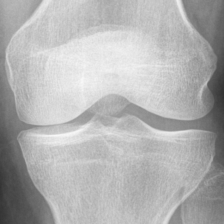
\includegraphics[width=\textwidth]{knee_0.png}
        \caption{KL 0}
        \label{fig:knee0}
    \end{subfigure}
    \hfill
    \begin{subfigure}[b]{0.19\textwidth}
        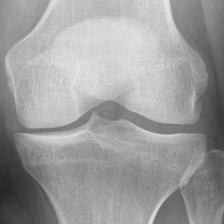
\includegraphics[width=\textwidth]{knee_1.png}
        \caption{KL 1}
        \label{fig:knee1}
    \end{subfigure}
    \hfill
    \begin{subfigure}[b]{0.19\textwidth}
        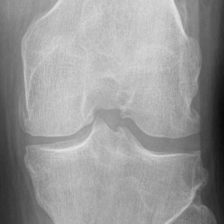
\includegraphics[width=\textwidth]{knee_2.png}
        \caption{KL 2}
        \label{fig:knee2}
    \end{subfigure}
    \hfill
    \begin{subfigure}[b]{0.19\textwidth}
        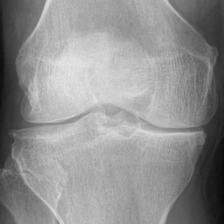
\includegraphics[width=\textwidth]{knee_3.png}
        \caption{KL 3}
        \label{fig:knee3}
    \end{subfigure}
    \hfill
    \begin{subfigure}[b]{0.19\textwidth}
        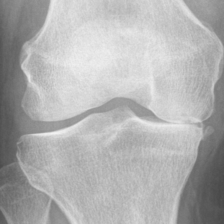
\includegraphics[width=\textwidth]{knee_4.png}
        \caption{KL 4}
        \label{fig:knee4}
    \end{subfigure}
    \caption{Ejemplos de radiografías de rodilla clasificadas según la escala Kellgren \& Lawrence (KL)}
    \label{fig:knee-examples}
\end{figure}



\section{--------Introducción---------}
En este capítulo se presenta una descripción exhaustiva del corpus utilizado para la detección y gradación de la artrosis en rodillas. Se abordan aspectos fundamentales relativos al dataset OAI, obtenido de Mendeley Data, así como la integración de elementos experimentales extraídos del paper \cite{efficientnet_paper}. En este contexto, se detallan los procesos de adquisición, preprocesamiento, análisis estadístico y organización en subconjuntos, elementos esenciales para el éxito en la aplicación de modelos de aprendizaje profundo.

\section{Adquisición y Descripción del Dataset OAI}
El dataset OAI se obtuvo de la plataforma Mendeley Data y se ha consolidado como una fuente de referencia para el estudio de la artrosis de rodilla. Este corpus se compone de radiografías que permiten evaluar la severidad de la enfermedad mediante el sistema de gradación de Kellgren-Lawrence (KL). Durante la fase de adquisición se integraron las clases \textit{test}, \textit{train}, \textit{val} y \textit{auto-test} presentadas en el dataset original, logrando el split empleado en \cite{efficientnet_paper}. Concretamente, el conjunto se redistribuyó en un 75\% para entrenamiento, 17\% para prueba y 8\% para validación.

\subsection{Distribución por Condición Médica y Estadísticas del Corpus}
En este trabajo, las clases se denominan de acuerdo con la condición médica asociada a la artrosis:
\begin{itemize}
    \item \textbf{Sin artrosis} (KL 0)
    \item \textbf{Leve} (KL 1)
    \item \textbf{Moderada} (KL 2)
    \item \textbf{Severa} (KL 3)
    \item \textbf{Muy severa} (KL 4)
\end{itemize}

La siguiente tabla resume la distribución numérica de imágenes en cada subconjunto:
\begin{center}
\begin{tabular}{lccccc}
\toprule
\textbf{Subconjunto} & \textbf{Sin artrosis} & \textbf{Leve} & \textbf{Moderada} & \textbf{Severa} & \textbf{Muy severa} \\
\midrule
\textit{auto-test} & 604 & 275 & 403 & 200 & 44 \\
\textit{train}     & 2286 & 1046 & 1516 & 757 & 173 \\
\textit{val}       & 328 & 153 & 212 & 106 & 27 \\
\textit{test}      & 639 & 296 & 447 & 223 & 51 \\
\bottomrule
\end{tabular}
\end{center}

Como complemento, se detallan a continuación los porcentajes de distribución por clase en cada
 subconjunto:

Conjunto de datos por clase
\begin{itemize}
    \item Sin artrosis: 39.5\%
    \item Leve: 18\%
    \item Moderada: 26.5\%
    \item Severa: 13\%
    \item Muy severa: 3\%
\end{itemize}
El corpus total se compone de 9786 imágenes, distribuidas en 1526 para auto-test, 5778 para entrenamiento, 826 para validación y 
1656 para prueba. Esta distribución y el equilibrio en las condiciones médicas son fundamentales para el entrenamiento y evaluación r
obusta de los modelos de clasificación.

\section{Preprocesamiento y Análisis del Corpus}
El preprocesamiento de las imágenes es una etapa crucial para asegurar la calidad y homogeneidad de los datos. Se aplicaron las siguientes técnicas:

\begin{itemize}
    \item \textbf{Redimensionamiento y Conversión a RGB:} Se ajustaron todas las imágenes a un tamaño uniforme de 224$\times$224 píxeles y se convirtieron al formato RGB, cumpliendo con las especificaciones de entrada de arquitecturas como EfficientNet.
    \item \textbf{Ecualización de Histograma:} Esta técnica se utilizó para mejorar el contraste, resaltando detalles fundamentales para la detección de patrones asociados a la artrosis.
    \item \textbf{Filtrado Bilateral:} Aplicado para suavizar las imágenes preservando bordes y detalles críticos, esenciales para la correcta interpretación anatómica.
    \item \textbf{Data Augmentation:} Se implementaron técnicas de aumento de datos (volteo horizontal y vertical) en el conjunto de entrenamiento, incrementando la variabilidad y robustez del modelo sin alterar la integridad de los conjuntos de validación y prueba.
\end{itemize}

El análisis estadístico del corpus resalta una distribución equilibrada entre las diferentes condiciones médicas, lo que es vital para el aprendizaje profundo y la posterior validación del modelo.

\section{Integración con el Paper}
El paper \cite{efficientnet_paper} utiliza el dataset OAI para evaluar un modelo ensemble basado en arquitecturas EfficientNet, mediante:

\begin{itemize}
    \item \textbf{Modelo Ensemble:} La combinación de EfficientNetB0 y EfficientNetB4 permite mejorar la precisión en la clasificación, aprovechando las fortalezas complementarias de cada arquitectura.
    \item \textbf{Estrategia de Entrenamiento:} Se han empleado pesos pre-entrenados junto con técnicas de regularización (Dropout y penalización L2) para optimizar la convergencia del modelo y minimizar el riesgo de sobreajuste.
    \item \textbf{Explainable AI:} La técnica Grad-CAM facilita la interpretación visual de las áreas críticas que influyen en las predicciones, aumentando la transparencia y confiabilidad del sistema.
\end{itemize}

La integración de estas metodologías, junto con el exhaustivo preprocesamiento y análisis del corpus, permite obtener resultados experimentales comparables con el estado del arte en la detección y gradación de la artrosis de rodilla.

\section{Conclusiones}
El análisis detallado del corpus del dataset OAI y su integración con las técnicas presentadas en \cite{efficientnet_paper} subraya la importancia de una adquisición y preprocesamiento minuciosos. La organización en subconjuntos, el equilibrio en la distribución de condiciones médicas y la aplicación de técnicas avanzadas en el tratamiento de imágenes sientan las bases para el desarrollo de modelos de aprendizaje profundo capaces de ofrecer diagnósticos precisos y fiables. Este enfoque contribuye significativamente al desarrollo de herramientas de asistencia al diagnóstico que combinan inteligencia artificial con técnicas de Explainable AI.

%%%%%%%%%%%%%%%%%%%%%%%%%%%%%%%%%%%%%%%%%%%%%%%%%%%%%%%%%%%%%%%%%%%%%%%%%%%%%%%


\chapter{Capítulo X | contribución 1: Experimentación y Análisis de Resultados}

\section{Introducción}
En este capítulo se presentan los experimentos realizados para evaluar el desempeño de diversas arquitecturas de redes neuronales en la detección de artrosis en rodillas. Con el objetivo de aportar evidencia empírica para la detección temprana de la enfermedad, se han probado variantes de modelos EfficientNet y ResNet utilizando dos estrategias de entrenamiento: el uso de pesos pre-entrenados (transfer learning) y el entrenamiento desde cero (\textit{from scratch}). Los experimentos se han llevado a cabo sobre el conjunto de datos Mendeley \cite{chen2018knee} y se han tomado como referencia las aportaciones teóricas y experimentales descritas en \cite{efficientnet_paper}. 

\section{Metodología Experimental}

\subsection{Configuración del Experimento}
Para todos los experimentos se siguió el siguiente protocolo:
\begin{itemize}
    \item \textbf{Preprocesamiento:} Se redimensionaron las imágenes a un tamaño uniforme (224x224), se aplicaron técnicas de histogram equalization y bilateral filtering y transformación de la imagen a RGB. Aparte de un aumentos de datos (flip horizontal y vertical) para mejorar la generalización del modelo.
    \item \textbf{Partición del Conjunto de Datos:} El dataset se dividió en subconjuntos de entrenamiento, validación y prueba, siguiendo los porcentajes previamente establecidos. 75\% para entrenamiento, 17\% para prueba y 8\% para validación.
    \item \textbf{Configuración de Entrenamiento:} Se usó la función de pérdida \textit{Categorical Cross-Entropy} y el optimizador Adam con una tasa de aprendizaje inicial de 0.001, aplicando un scheduler para la reducción de la tasa en caso de estancamiento. Se entrenó hasta 50 épocas, implementando técnicas de Early Stopping para evitar sobreajuste. También se aplicó regularización L2 con valores entre 0.001 y 0.0001 para prevenir el sobreajuste.
\end{itemize}

\subsection{Modelos Evaluados}
Se evaluaron las siguientes arquitecturas:
\begin{itemize}
    \item \textbf{EfficientNet:} De la familia se probaron los modelos B0, B4, B5 y B7
    \item \textbf{ResNet50:} Modelo representativo de la familia ResNet.
\end{itemize}

\subsection{Estrategias de Entrenamiento}
Se compararon dos enfoques:
\begin{enumerate}
    \item \textbf{Transfer Learning:} Utilizando pesos pre-entrenados en grandes bases de datos (por ejemplo, ImageNet) para adaptar el modelo a la tarea específica de clasificación de artrosis.
    \item \textbf{Entrenamiento Desde Cero (\textit{From Scratch}):} Inicializando los pesos de manera aleatoria y entrenando la red sin conocimiento previo.
\end{enumerate}

\section{Resultados Experimentales}

\subsection{Comparación de Arquitecturas y Estrategias}
Los experimentos demostraron que, en su mayoría, tanto los modelos EfficientNet como los ResNet alcanzaron precisiones cercanas al 70\%, excepto EfficientNetB5 que logró una precisión del 71\%. La Tabla \ref{tab:resultados_experimentos} resume los resultados obtenidos.
La precisión obtenida se escogió en base a la época de entrenamiento con menor pérdida. En algunos casos los modelos conseguian una mejor precisión con mayor perdida, pero no siendo significativa la mejora.
\begin{table}[htbp]
\centering
\begin{tabular}{lccc}
\toprule
\textbf{Modelo y Estrategia} & \textbf{Precisión (\%)} & \textbf{Val loss} & \textbf{Épocas necesarias} \\
\midrule
EfficientNetB0 (Pre-entrenado)  & 69.87\%    & 0.73 & 7 \\
EfficientNetB5 (Pre-entrenado)  & 72.82\%    & 0.81 & 2 \\
EfficientNetB7 (Pre-entrenado)  & 66.54\%    & 0.79 & 13 \\
EfficientNetB4 (Desde Cero)     & 59.36\%    & 0.96 & 49 \\
ResNet50 (Pre-entrenado)        & 66.66\%    & 0.78 & 4 \\
ResNet50 (Desde Cero)           & 65.89\%    & 0.84 & 28 \\

\bottomrule
\end{tabular}
\caption{Comparación de modelos y estrategias de entrenamiento}
\label{tab:resultados_experimentos}
\end{table}

\begin{figure}[htbp]
    \centering
    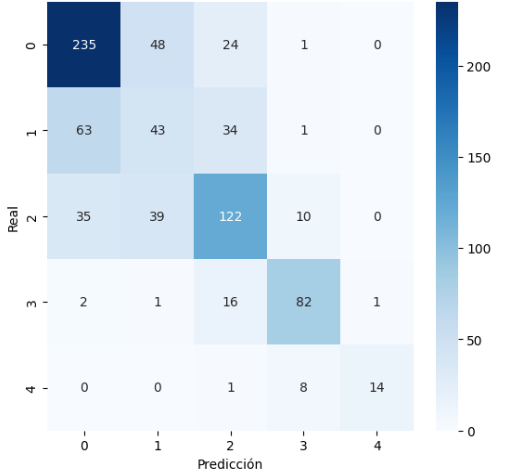
\includegraphics[width=0.6\textwidth]{EfficientNet_B7.png}
    \caption{Descripción de la imagen}
    \label{fig:matriz_confusion}
\end{figure}

\subsection{Impacto del Uso de Pesos Pre-entrenados}
Los experimentos evidenciaron que:
\begin{itemize}
    \item \textbf{Convergencia Rápida:} Los modelos con pesos pre-entrenados alcanzaron la convergencia en menos épocas, reduciendo significativamente el tiempo de entrenamiento.
    \item \textbf{Mayor Precisión:} Se observó un aumento en la precisión (hasta 71\% en el caso de EfficientNetB5) en comparación con el entrenamiento desde cero, donde los resultados se situaron en torno al 67-68\%.
    \item \textbf{Robustez del Modelo:} Los modelos pre-entrenados realizaban un overfitting mas pronunciado, pero la precisión obtenida era mayor que los modelos entrenados desde cero.
\end{itemize}

\subsection{Análisis Comparativo y Discusión}
La comparación entre los dos enfoques de entrenamiento resalta la importancia de la transferencia de aprendizaje en el dominio biomédico:
\begin{itemize}
    \item Aunque la mejora en precisión entre modelos pre-entrenados y entrenados desde cero es modesta (aproximadamente un 1-2\%), esta diferencia es crucial en aplicaciones clínicas, donde cada punto porcentual puede tener un impacto significativo en el diagnóstico.
    \item El entrenamiento desde cero presentó desventajas claras, tales como un mayor consumo de recursos computacionales y un tiempo de entrenamiento considerablemente más largo, lo cual puede ser prohibitivo en entornos con recursos limitados.
    \item EfficientNetB5 destacó frente a las demás arquitecturas, lo que sugiere que una mayor capacidad del modelo (a pesar de aumentar la complejidad) puede traducirse en mejoras en el desempeño, siempre y cuando se disponga de una estrategia de entrenamiento adecuada.
\end{itemize}

\section{Conclusiones del Capítulo}
Los experimentos realizados permiten concluir que:

\cleardoublepage


\chapter{Capítulo 2 de contribución}   % ~15 páginas
% Expón aquí tu segundo objetivo y resultados derivados

%%%%%%%%%%%%%%%%%%%%%%%%%%%%%%%%%%%%%%%%%%%%%%%%%%%%%%%%%%%%%%%%%%%%%%%%%%%%%%%
%                              CAPÍTULO 5                                     %
%                     TERCERA CONTRIBUCIÓN (OBJETIVO 3)                       %
%%%%%%%%%%%%%%%%%%%%%%%%%%%%%%%%%%%%%%%%%%%%%%%%%%%%%%%%%%%%%%%%%%%%%%%%%%%%%%%

\chapter{Capítulo 3 de contribución}   % ~15 páginas
% Expón aquí tu tercer objetivo y resultados derivados

%%%%%%%%%%%%%%%%%%%%%%%%%%%%%%%%%%%%%%%%%%%%%%%%%%%%%%%%%%%%%%%%%%%%%%%%%%%%%%%
%                              CAPÍTULO 6                                     %
%                                CONCLUSIONES                                 %
%%%%%%%%%%%%%%%%%%%%%%%%%%%%%%%%%%%%%%%%%%%%%%%%%%%%%%%%%%%%%%%%%%%%%%%%%%%%%%%

\chapter{Conclusiones}  % ~5 páginas

\section{Resumen del trabajo realizado} % 6.1
% Repasa y sintetiza las secciones principales

\section{Objetivos alcanzados}         % 6.2
% Verifica si se cumplieron los objetivos planteados

\section{Trabajo futuro}               % 6.3
% Explica las posibles extensiones o mejoras

%%%%%%%%%%%%%%%%%%%%%%%%%%%%%%%%%%%%%%%%%%%%%%%%%%%%%%%%%%%%%%%%%%%%%%%%%%%%%%%
%                              BIBLIOGRAFÍA                                   %
%%%%%%%%%%%%%%%%%%%%%%%%%%%%%%%%%%%%%%%%%%%%%%%%%%%%%%%%%%%%%%%%%%%%%%%%%%%%%%%

\printbibliography 
\cleardoublepage

%%%%%%%%%%%%%%%%%%%%%%%%%%%%%%%%%%%%%%%%%%%%%%%%%%%%%%%%%%%%%%%%%%%%%%%%%%%%%%%
%                           APÉNDICES (OPCIONALES)                            %
%%%%%%%%%%%%%%%%%%%%%%%%%%%%%%%%%%%%%%%%%%%%%%%%%%%%%%%%%%%%%%%%%%%%%%%%%%%%%%%

\APPENDIX

\chapter{Configuración del sistema}
% ...

\chapter{Otro apéndice}
% ...

\end{document}
